\documentclass[a4paper]{article}
\usepackage{cmap}
\usepackage[utf8]{inputenc}
\usepackage[T2A]{fontenc}
\usepackage[english,russian]{babel} 
\usepackage[left=15mm, top=15mm, right=15mm, bottom=42mm, nohead, nofoot]{geometry}
\usepackage{blindtext}  % рыба-текст
\usepackage{graphicx}  % изобржаения
\usepackage{float} % плавающие объекты
\usepackage{wrapfig}  % изобржаения
\usepackage{tikz} % графика
\usepackage{xcolor} % определение цветов
\usepackage{nicefrac} % красивые дроби
\usepackage{cancel} % сокращение
\usepackage{amsmath,amsfonts,amssymb} % математический пакет
\usepackage{hyperref}  % гиперссылки
\usepackage{fancybox,fancyhdr} % хедер и футер
\usepackage{listings} % код
\usepackage{accsupp}
\pagestyle{fancy}
\fancyhf{}
\fancyhead[L]{Лабораторная работа №5}
\fancyhead[R]{\textit{Связь непрерывного и дискретного}}
\fancyfoot[C]{\thepage}
\headsep=8mm
\footskip=20mm

\definecolor{urlcolor}{HTML}{3454D1}
\definecolor{linkcolor}{HTML}{3454D1}
\hypersetup{pdfstartview=FitH, linkcolor=linkcolor, urlcolor=urlcolor, colorlinks=true}

\definecolor{strings}{rgb}{0,0.6,0}
\definecolor{comments}{rgb}{0,0.3,0}
\definecolor{numbers}{rgb}{0.5,0.5,0.5}
\definecolor{keywords}{rgb}{0.09,0.61,0.95}
\definecolor{background}{rgb}{0.97,0.97,0.97}
\newcommand{\noncopynumber}[1]{%
    \BeginAccSupp{method=escape,ActualText={}}%
    #1%
    \EndAccSupp{}%
}
\lstdefinestyle{codestyle}{
    backgroundcolor=\color{background},
    commentstyle=\color{comments},
    keywordstyle=\color{keywords},
    stringstyle=\color{strings},
    numberstyle=\tiny\color{numbers}\noncopynumber,
    basicstyle=\ttfamily\footnotesize,
    breakatwhitespace=false,
    breaklines=true,
    captionpos=b,
    inputencoding=utf8,
    keepspaces=true,
    numbers=left,
    numbersep=5pt,
    showspaces=false,
    showstringspaces=false,
    showtabs=false,
    tabsize=2,
    extendedchars=true,
    literate=
    {а}{{\cyra}}1
    {б}{{\cyrb}}1
    {в}{{\cyrv}}1
    {г}{{\cyrg}}1
    {д}{{\cyrd}}1
    {е}{{\cyre}}1
    {ж}{{\cyrzh}}1
    {з}{{\cyrz}}1
    {и}{{\cyri}}1
    {й}{{\cyrishrt}}1
    {к}{{\cyrk}}1
    {л}{{\cyrl}}1
    {м}{{\cyrm}}1
    {н}{{\cyrn}}1
    {о}{{\cyro}}1
    {п}{{\cyrp}}1
    {р}{{\cyrr}}1
    {с}{{\cyrs}}1
    {т}{{\cyrt}}1
    {у}{{\cyru}}1
    {ф}{{\cyrf}}1
    {х}{{\cyrh}}1
    {ц}{{\cyrc}}1
    {ч}{{\cyrch}}1
    {ш}{{\cyrsh}}1
    {щ}{{\cyrshch}}1
    {ъ}{{\cyrhrdsn}}1
    {ы}{{\cyrery}}1
    {ь}{{\cyrsftsn}}1
    {э}{{\cyrerev}}1
    {ю}{{\cyryu}}1
    {я}{{\cyrya}}1
    {А}{{\CYRA}}1
    {Б}{{\CYRB}}1
    {В}{{\CYRV}}1
    {Г}{{\CYRG}}1
    {Д}{{\CYR96}}1
    {Е}{{\CYRE}}1
    {Ж}{{\CYRZH}}1
    {З}{{\CYRZ}}1
    {И}{{\CYRI}}1
    {Й}{{\CYRISHRT}}1
    {К}{{\CYRK}}1
    {Л}{{\CYRL}}1
    {М}{{\CYRM}}1
    {Н}{{\CYRN}}1
    {О}{{\CYRO}}1
    {П}{{\CYRP}}1
    {Р}{{\CYRR}}1
    {С}{{\CYRS}}1
    {Т}{{\CYRT}}1
    {У}{{\CYRU}}1
    {Ф}{{\CYRF}}1
    {Х}{{\CYRH}}1
    {Ц}{{\CYRC}}1
    {Ч}{{\CYRCH}}1
    {Ш}{{\CYRSH}}1
    {Щ}{{\CYRSHCH}}1
    {Ъ}{{\CYRHRDSN}}1
    {Ы}{{\CYRERY}}1
    {Ь}{{\CYRSFTSN}}1
    {Э}{{\CYREREV}}1
    {Ю}{{\CYRYU}}1
    {Я}{{\CYRYA}}1
}

\lstset{style=codestyle}

\addto\captionsrussian{
  \renewcommand{\contentsname}
    {\centering Содержание}
}


\newlength{\tempheight}
\newcommand{\Let}{
\mathbin{\text{\settoheight{\tempheight}{\mathstrut}\raisebox{0.4\pgflinewidth}{
\tikz[baseline=0.5ex,line cap=round,line join=round] \draw (0,0) --++ (0.3em,0) --++ (0,2.3ex) --++ (-0.3em,0);
}}}}
\newcommand*\squared[1]{\tikz[baseline=(char.base)]{
            \node[shape=rectangle,draw,inner sep=4pt] (char) {#1};}}
\newcommand*\msquared[1]{\tikz[baseline=(char.base)]{
            \node[shape=rectangle,draw,inner sep=4pt] (char) {$\displaystyle #1$};}}
\newcommand{\at}{\biggr\rvert}
\newcommand{\shiftright}[3]{\makebox[#2][r]{\makebox[#1][l]{#3}}}
\newcommand{\e}{\;\text{e}}
\let\oldint\int
\def\int{\oldint\limits}
\DeclareRobustCommand{\divby}{%
  \mathrel{\vbox{\baselineskip.65ex\lineskiplimit0pt\hbox{.}\hbox{.}\hbox{.}}}%
}

\newcommand\NB{\textbf{N\kern-0.32em\textcolor{red}{B}}}

\begin{document}

\begin{titlepage}
    \begin{center}
        Федеральное государственное автономное образовательное \\ учреждение высшего образования \\[6pt]
        САНКТ-ПЕТЕРБУРГСКИЙ НАЦИОНАЛЬНЫЙ \\ ИССЛЕДОВАТЕЛЬСКИЙ УНИВЕРСИТЕТ ИТМО \\[16pt]
        Факультет систем управления и робототехники \\[26em]
        Лабораторная работа №5 \\[0.5em]
        \textbf{СВЯЗЬ НЕПРЕРЫВНОГО И ДИСКРЕТНОГО}
    \end{center}\,\\[10em]
    \begin{flushright}
        Студент: Заводин Е.Ю.\\
        Поток: ЧастМет R23 1.6 \\[0.5em]
        Преподаватели: Перегудин А.А.\\
        Догадин Е.В.
    \end{flushright}\,\\[6em]
    \begin{center}
        {\small Санкт-Петербург \\ 2025}
    \end{center}
\end{titlepage}
\setcounter{page}{2}
\tableofcontents\newpage

\section{Непрерывное и дискретное преобразование Фурье}\

Рассмотрим прямоугольную функцию $\Pi : \mathbb{R} \to \mathbb{R} :$

$$
\Pi(t) = \begin{cases}
    1, & \left| t \right| \leq 1/2, \\
    0, & \left| t \right| > 1/2.
\end{cases}
$$\

Найдем её Фурье-образ аналитически:

$$
\hat{\Pi}(\nu) = \int_{-\infty}^{+\infty} \Pi(t) e^{-2\pi i \nu t}\, dt = \int_{-1/2}^{1/2} 1 \cdot e^{-2\pi i \nu t} \, dt = \Bigg [ u = -2i\pi \nu t \Rightarrow du = -2i \pi \nu \, dt \Bigg ] = \frac{i}{2\pi \nu} \int_{-1/2}^{1/2} e^u \, du =$$
$$= \frac{i}{2\pi \nu} e^u \Bigg |^{1/2}_{-1/2} =\frac{i e^{-2i\pi \nu t}}{2\pi \nu} \Bigg |^{1/2}_{-1/2} = \frac{\sin{(\pi \nu)}}{\pi\nu} = \mathrm{sinc} (\pi\nu).
$$\ 

Посмотрим на графики функции и полученного Фурье-образа:

\begin{figure}[H]
    \begin{minipage}{0.5\textwidth}
        \centering \includegraphics[width=\textwidth]{graphs/func.png}
        \caption{Прямоугольная функция}
    \end{minipage}\hfill
    \begin{minipage}{0.5\textwidth}
        \centering \includegraphics[width=\textwidth]{graphs/fourier.png}
        \caption{Фурье-образ прямоугольной функции}
    \end{minipage}\\[1em]
\end{figure}\noindent\

\subsection{Численное интегрирование}\

Построим график Фурье-образа без аналитического расчёта интеграла, путём численного интегрирования с использование функции frapz в Matlab:

\begin{figure}[H]
    \centering
    \includegraphics[width=0.55\linewidth]{graphs/fourier_numerical.png}
    \caption{Фурье-образ прямоугольной функции (численное интегрирование)}
\end{figure}

Далее выполним обратное преобразование Фурье путём использования той же функции, поменяв лишь сам интеграл, подаваемый в неё:

\begin{figure}[H]
    \centering
    \includegraphics[width=0.55\linewidth]{graphs/func_inversed_fourier.png}
    \caption{Восстановленная обратным преобразованием Фурье функция}
\end{figure}

Заметны гиббсовские осцилляции, попробуем избавиться от них при помощи подбора более подходящих значений параметров $T, dt, V, dv$. Результат преобразования Фурье вычислялся дольше, чем при использовании функции FFT, впредь буду замерять это время. Уменьшим в 2 раза промежуток интегрирования по частоте $V$, посмотрим на изменения на получившемся наборе параметров $V = 12, T = 4, \Delta t=\Delta \nu=0.001$:

\begin{figure}[H]
    \begin{minipage}{0.5\textwidth}
        \centering \includegraphics[width=\textwidth]{graphs/1/T_4_dt_0.001_V_12_dv_0.001/fourier_numerical.png}
        \caption{Фурье-образ прямоугольной функции}
    \end{minipage}\hfill
    \begin{minipage}{0.5\textwidth}
        \centering \includegraphics[width=\textwidth]{graphs/1/T_4_dt_0.001_V_12_dv_0.001/func_inversed_fourier.png}
        \caption{Восстановленная обратным преобразованием Фурье функция}
    \end{minipage}\\[1em]
\end{figure}\noindent\

Затраченное время составило 3.23 секунд для нахождения результата прямого преобразования Фурье. Видно, что на обоих графиках частота колебаний стала меньше, что похоже на взятие меньшего количества первых членов частичных сумм ряда Фурье (качественно методы разные, ведь там конечная сумма, а тут интеграл), так как рассматривается меньшее количество частот. Возьмём $V = 48$, частота колебаний должна увеличиться:

\begin{figure}[H]
    \begin{minipage}{0.5\textwidth}
        \centering \includegraphics[width=\textwidth]{graphs/1/T_4_dt_0.001_V_48_dv_0.001/fourier_numerical.png}
        \caption{Фурье-образ прямоугольной функции}
    \end{minipage}\hfill
    \begin{minipage}{0.5\textwidth}
        \centering \includegraphics[width=\textwidth]{graphs/1/T_4_dt_0.001_V_48_dv_0.001/func_inversed_fourier.png}
        \caption{Восстановленная обратным преобразованием Фурье функция}
    \end{minipage}\\[1em]
\end{figure}\noindent\

Время нахождения прямого преобразования сильно возросло -- 13.52 секунды, однако функция стала больше похожа на исходную. Теперь изменим $dv$, и посмотрим на результат на наборе параметров $V = 15, T = 10, \Delta t = 0.001, \Delta \nu=0.3$:

\begin{figure}[H]
    \begin{minipage}{0.5\textwidth}
        \centering \includegraphics[width=\textwidth]{graphs/1/T_10_dt_0.001_V_15_dv_0.3/fourier_numerical.png}
        \caption{Фурье-образ прямоугольной функции}
    \end{minipage}\hfill
    \begin{minipage}{0.5\textwidth}
        \centering \includegraphics[width=\textwidth]{graphs/1/T_10_dt_0.001_V_15_dv_0.3/func_inversed_fourier.png}
        \caption{Восстановленная обратным преобразованием Фурье функция}
    \end{minipage}\\[1em]
\end{figure}\noindent\

Заметно, что график Фурье-образа функции теперь имеет изломы, а сама функция получила периодическое продолжение, как это происходило при рассмотрении приближении функций рядами Фурье на ограниченном промежутке. Образ Фурье же был вычислен за 0.05 секунды. Ещё увеличим шаг частот, примем $\Delta \nu = 0.5$: 

\begin{figure}[H]
    \begin{minipage}{0.5\textwidth}
        \centering \includegraphics[width=\textwidth]{graphs/1/T_10_dt_0.001_V_15_dv_0.5/fourier_numerical.png}
        \caption{Фурье-образ прямоугольной функции}
    \end{minipage}\hfill
    \begin{minipage}{0.5\textwidth}
        \centering \includegraphics[width=\textwidth]{graphs/1/T_10_dt_0.001_V_15_dv_0.5/func_inversed_fourier.png}
        \caption{Восстановленная обратным преобразованием Фурье функция}
    \end{minipage}\\[1em]
\end{figure}\noindent\

Изломов на Фурье-образе стало больше, а сама функция стала повторяться чаще, что в сравнении с преобразованием Фурье на конечном промежутке аналогично уменьшению промежутка, на котором рассматривается функция. Разумеется, с увеличением значения $\Delta \nu$ растёт быстродействие (время выполнения кода -- 0.03 секунды) и падает точность.\ 
Выясним влияние размера интегрируемого по времени промежутка $T$. Примем набор параметров $V = 12, T = 0.8, \Delta t = 0.001, \Delta \nu=0.001$, посмотрим на сравнительные графики:

\begin{figure}[H]
    \begin{minipage}{0.5\textwidth}
        \centering \includegraphics[width=\textwidth]{graphs/1/T_0.8_dt_0.001_V_12_dv_0.001/fourier_numerical.png}
        \caption{Фурье-образ прямоугольной функции}
    \end{minipage}\hfill
    \begin{minipage}{0.5\textwidth}
        \centering \includegraphics[width=\textwidth]{graphs/1/T_0.8_dt_0.001_V_12_dv_0.001/func_inversed_fourier.png}
        \caption{Восстановленная обратным преобразованием Фурье функция}
    \end{minipage}\\[1em]
\end{figure}\noindent\

Образ функции был вычислен за 0.82 секунды. Для $T = 2$:

\begin{figure}[H]
    \begin{minipage}{0.5\textwidth}
        \centering \includegraphics[width=\textwidth]{graphs/1/T_2_dt_0.001_V_12_dv_0.001/fourier_numerical.png}
        \caption{Фурье-образ прямоугольной функции}
    \end{minipage}\hfill
    \begin{minipage}{0.5\textwidth}
        \centering \includegraphics[width=\textwidth]{graphs/1/T_2_dt_0.001_V_12_dv_0.001/func_inversed_fourier.png}
        \caption{Восстановленная обратным преобразованием Фурье функция}
    \end{minipage}\\[1em]
\end{figure}\noindent\

Образ функции был вычислен за 1.81 секунды. Для $T = 20$:

\begin{figure}[H]
    \begin{minipage}{0.5\textwidth}
        \centering \includegraphics[width=\textwidth]{graphs/1/T_20_dt_0.001_V_12_dv_0.001/fourier_numerical.png}
        \caption{Фурье-образ прямоугольной функции}
    \end{minipage}\hfill
    \begin{minipage}{0.5\textwidth}
        \centering \includegraphics[width=\textwidth]{graphs/1/T_20_dt_0.001_V_12_dv_0.001/func_inversed_fourier.png}
        \caption{Восстановленная обратным преобразованием Фурье функция}
    \end{minipage}\\[1em]
\end{figure}\noindent\

Образ функции был вычислен за 18.45 секунд. Для $T = 100$:

\begin{figure}[H]
    \begin{minipage}{0.5\textwidth}
        \centering \includegraphics[width=\textwidth]{graphs/1/T_100_dt_0.001_V_12_dv_0.001/fourier_numerical.png}
        \caption{Фурье-образ прямоугольной функции}
    \end{minipage}\hfill
    \begin{minipage}{0.5\textwidth}
        \centering \includegraphics[width=\textwidth]{graphs/1/T_100_dt_0.001_V_12_dv_0.001/func_inversed_fourier.png}
        \caption{Восстановленная обратным преобразованием Фурье функция}
    \end{minipage}\\[1em]
\end{figure}\noindent\

В этот раз образ функции был найден за 84.33 секунды.

Визуально ни график Фурье-образа, ни график восстановленной функции не меняется при изменении $T$ (при $T$ > 1, иначе рассматриваемый промежуток не захватывает точки, в которых функция меняет значение с 0 на 1, и образ не сходится к кардинальному синусу), меняется лишь время, затрачиваемое на выполнение -- чем выше $T$, тем медленнее программа производит расчёты.\ 
Теперь посмотрим на влияние $\Delta t$. Рассмотрим набор параметров $V = 12, T = 10, \Delta t = 0.05, \Delta \nu=0.001$:

\begin{figure}[H]
    \begin{minipage}{0.5\textwidth}
        \centering \includegraphics[width=\textwidth]{graphs/1/T_10_dt_0.05_V_12_dv_0.001/fourier_numerical.png}
        \caption{Фурье-образ прямоугольной функции}
    \end{minipage}\hfill
    \begin{minipage}{0.5\textwidth}
        \centering \includegraphics[width=\textwidth]{graphs/1/T_10_dt_0.05_V_12_dv_0.001/func_inversed_fourier.png}
        \caption{Восстановленная обратным преобразованием Фурье функция}
    \end{minipage}\\[1em]
\end{figure}\noindent\

Образ функции был вычислен за 0.41 секунд. При $\Delta t = 0.1$:

\begin{figure}[H]
    \begin{minipage}{0.5\textwidth}
        \centering \includegraphics[width=\textwidth]{graphs/1/T_10_dt_0.1_V_12_dv_0.001/fourier_numerical.png}
        \caption{Фурье-образ прямоугольной функции}
    \end{minipage}\hfill
    \begin{minipage}{0.5\textwidth}
        \centering \includegraphics[width=\textwidth]{graphs/1/T_10_dt_0.1_V_12_dv_0.001/func_inversed_fourier.png}
        \caption{Восстановленная обратным преобразованием Фурье функция}
    \end{minipage}\\[1em]
\end{figure}\noindent\

Образ функции был вычислен за 0.30 секунд. При $\Delta t = 0.25$:

\begin{figure}[H]
    \begin{minipage}{0.5\textwidth}
        \centering \includegraphics[width=\textwidth]{graphs/1/T_10_dt_0.25_V_12_dv_0.001/fourier_numerical.png}
        \caption{Фурье-образ прямоугольной функции}
    \end{minipage}\hfill
    \begin{minipage}{0.5\textwidth}
        \centering \includegraphics[width=\textwidth]{graphs/1/T_10_dt_0.25_V_12_dv_0.001/func_inversed_fourier.png}
        \caption{Восстановленная обратным преобразованием Фурье функция}
    \end{minipage}\\[1em]
\end{figure}\noindent\

Образ функции был вычислен за 0.26 секунд. При $\Delta t = 0.5$:

\begin{figure}[H]
    \begin{minipage}{0.5\textwidth}
        \centering \includegraphics[width=\textwidth]{graphs/1/T_10_dt_0.5_V_12_dv_0.001/fourier_numerical.png}
        \caption{Фурье-образ прямоугольной функции}
    \end{minipage}\hfill
    \begin{minipage}{0.5\textwidth}
        \centering \includegraphics[width=\textwidth]{graphs/1/T_10_dt_0.5_V_12_dv_0.001/func_inversed_fourier.png}
        \caption{Восстановленная обратным преобразованием Фурье функция}
    \end{minipage}\\[1em]
\end{figure}\noindent\

Образ функции был вычислен за 0.22 секунды. 

Видим, что увеличение шага по времени приводит к сильным расхождениям графиков восстановленной функции и оригинала, и график восстановленной функции становится грубым. Время же, затрачиваемое на работу метода, уменьшается с увеличением $\Delta t$.

\subsubsection{Выводы}\

Увеличение величины шага позитивно сказывается на быстродействии метода, однако негативно влияет на его точность, увеличение размера промежутка плохо отражается на быстродействии, и в случае с промежутком интегрирования по времени не приводит к изменению точности (если брать промежуток в разумных пределах, в которых функция значима), в случае с промежутком интегрирования по частоте приводит к повышению точности, однако плохо сказывается на быстродействии -- для достижения наилучших результатов нужно искать баланс.

\subsection{Использование DFT}\

Теперь попробуем использовать унитарное дискретное преобразование, искать образ будем по следующей формуле: 

$$
\hat{f}(\nu_m) = \frac{1}{\sqrt{N}} \sum_{n=0}^{N-1} f(t_n) \e^{-2\pi i (\frac{mn}{N})}
$$\

Результат обратного преобразования же будет найден следующим образом:

$$
x_n = \mathcal{F}^{-1}\{\hat{f}(\nu_m)\} = \frac{1}{\sqrt{N}} \sum_{n=0}^{N-1} \hat{f}(\nu_m) \e^{2\pi i (\frac{mn}{N})}
$$

Сначала рассмотрим действие дискретного преобразования Фурье при $T = 100, \Delta t = 0.001, V = 1/\Delta t = 1000, \Delta \nu = 1/T = 0.01$:

\begin{figure}[H]
    \begin{minipage}{0.5\textwidth}
        \centering \includegraphics[width=\textwidth]{graphs/2/T_100_dt_0.001_V_1000_dv_0.01/fourier_numerical.png}
        \caption{Фурье-образ прямоугольной функции}
    \end{minipage}\hfill
    \begin{minipage}{0.5\textwidth}
        \centering \includegraphics[width=\textwidth]{graphs/2/T_100_dt_0.001_V_1000_dv_0.01/func_inversed_fourier.png}
        \caption{Восстановленная обратным преобразованием Фурье функция}
    \end{minipage}\\[1em]
\end{figure}\noindent\

Затраченное время составило 0.004 секунды.

При увеличении $\Delta t$ уменьшается амплитуда Фурье-образа функции и наблюдается небольшое отклонение восстановленной функции от исходной, это отклонение увеличивается по мере роста $\Delta t$, так как соразмерно с ростом значения этого параметра уменьшается промежуток частот $V = 1/\Delta t$. Вот графики, подтверждающие это:\

При $\Delta t = 0.1$ ($V = 10$):

\begin{figure}[H]
    \begin{minipage}{0.5\textwidth}
        \centering \includegraphics[width=\textwidth]{graphs/2/T_100_dt_0.1_V_10_dv_0.01/fourier_numerical.png}
        \caption{Фурье-образ прямоугольной функции}
    \end{minipage}\hfill
    \begin{minipage}{0.5\textwidth}
        \centering \includegraphics[width=\textwidth]{graphs/2/T_100_dt_0.1_V_10_dv_0.01/func_inversed_fourier.png}
        \caption{Восстановленная обратным преобразованием Фурье функция}
    \end{minipage}\\[1em]
\end{figure}\noindent\

Затраченное время составило 0.001 секунды. При $\Delta t = 0.5$ ($V = 2$):

\begin{figure}[H]
    \begin{minipage}{0.5\textwidth}
        \centering \includegraphics[width=\textwidth]{graphs/2/T_100_dt_0.5_V_2_dv_0.01/fourier_numerical.png}
        \caption{Фурье-образ прямоугольной функции}
    \end{minipage}\hfill
    \begin{minipage}{0.5\textwidth}
        \centering \includegraphics[width=\textwidth]{graphs/2/T_100_dt_0.5_V_2_dv_0.01/func_inversed_fourier.png}
        \caption{Восстановленная обратным преобразованием Фурье функция}
    \end{minipage}\\[1em]
\end{figure}\noindent\

Затраченное время составило 0.034 секунды. 
При уменьшении параметра $T$ увеличивается $\Delta \nu$, на графиках Фурье-образов растёт амплитуда и увеличивается расстояние между точками, в которых вычисляются значения образов, а графики восстановленной функции почти не меняются -- зафиксируем $\Delta t = 0.001$, тогда:

При $T = 10$ ($\Delta \nu = 0.1$):

\begin{figure}[H]
    \begin{minipage}{0.5\textwidth}
        \centering \includegraphics[width=\textwidth]{graphs/2/T_10_dt_0.001_V_1000_dv_0.1/fourier_numerical.png}
        \caption{Фурье-образ прямоугольной функции}
    \end{minipage}\hfill
    \begin{minipage}{0.5\textwidth}
        \centering \includegraphics[width=\textwidth]{graphs/2/T_10_dt_0.001_V_1000_dv_0.1/func_inversed_fourier.png}
        \caption{Восстановленная обратным преобразованием Фурье функция}
    \end{minipage}\\[1em]
\end{figure}\noindent\

Затраченное время составило 0.001 секунды. При $T = 1.5$ ($\Delta \nu = 2/3$):

\begin{figure}[H]
    \begin{minipage}{0.5\textwidth}
        \centering \includegraphics[width=\textwidth]{graphs/2/T_1.5_dt_0.001_V_1000_dv_0.66667/fourier_numerical.png}
        \caption{Фурье-образ прямоугольной функции}
    \end{minipage}\hfill
    \begin{minipage}{0.5\textwidth}
        \centering \includegraphics[width=\textwidth]{graphs/2/T_1.5_dt_0.001_V_1000_dv_0.66667/func_inversed_fourier.png}
        \caption{Восстановленная обратным преобразованием Фурье функция}
    \end{minipage}\\[1em]
\end{figure}\noindent\

Затраченное время составило 0.033 секунды. При $T = 0.8$ ($\Delta \nu = 1.25$):

\begin{figure}[H]
    \begin{minipage}{0.5\textwidth}
        \centering \includegraphics[width=\textwidth]{graphs/2/T_0.8_dt_0.001_V_1000_dv_1.25/fourier_numerical.png}
        \caption{Фурье-образ прямоугольной функции}
    \end{minipage}\hfill
    \begin{minipage}{0.5\textwidth}
        \centering \includegraphics[width=\textwidth]{graphs/2/T_0.8_dt_0.001_V_1000_dv_1.25/func_inversed_fourier.png}
        \caption{Восстановленная обратным преобразованием Фурье функция}
    \end{minipage}\\[1em]
\end{figure}\noindent\

Затраченное время составило 0.011 секунды. 

\subsubsection{Выводы}\

Метод работает гораздо быстрее, что позволяет выбирать большие промежутки интегрирования одновременно с малыми величинами шага. Взятие слишком больших $\Delta t$ приводит к уменьшению $V$, за счет чего восстановленная функция начинает слабо походить на прямоугольную, однако с рассмотренными в этом пункте значениями параметра $\Delta t$ при численном интегрировании получился бы куда более плохой результат. Использование малых $T$ почти никак не меняет функцию, даже в случае $2\,T < 1$, хотя, казалось бы, в этом случае ``значащая'' часть функции не полностью входит в рассматриваемый промежуток. Однако, при такой прекрасной сходимости восстановленной функции с исходной при малых временных затратах, образ вовсе не похож на тот, что был найден аналитически.

\subsection{Объяснения}\

Численное интегрирование при помощи trapz -- именно интегрирование (отображение непрерывного в непрерывное, хоть и с ограничением в виде машинной точности), и в его результате получается непрерывная функция -- именно тот приближенный интеграл, который и получается в результате аналитического нахождения. А при использовании DFT выполняется суммирование, которое не сходится к интегралу, найденному аналитически -- его природа другая. Скорость выполнения FFT выше, чем frapz -- на то FFT и Fast Fourier Transform, потому что быстрый, ведь оптимизирован он так, что его вычислительная сложность меньше, чем при нахождении образа Фурье численном интегрированием ($O(N \log N)$ против $O(N^2)$).

\subsection{Приближение непрерывного с помощью DFT}\

Попытаемся воссоздать непрерывный Фурье-образ с помощью дискретной формы преобразования Фурье. Для этого аппроксимируем непрерывное преобразование Фурье на конечном промежутке $T = b - a$ суммой Римана:

$$
\hat{f}(\nu) \approx \int_{-T/2}^{T/2} f(t) e^{-2\pi i\nu t} \, dt; \hat{f}(\nu_m) \approx \sum_{n=0}^{N-1} f(t_n) e^{-2\pi i \nu_m t_n} \Delta t.
$$\ 

С учетом $t_n = \frac{T}{2} + n\Delta t$:

$$
\hat{f}(\nu_m) \approx \sum_{n = 0}^{N - 1} f(t_n)e^{-2\pi i \frac{m}{T} (\frac{T}{2} + n\Delta t)}\Delta t = \sum_{n = 0}^{N - 1} f(t_n)e^{-\pi i m -2\pi i \frac{mn\Delta t}{T}} \Delta t = \sum_{n = 0}^{N - 1} f(t_n)e^{-\pi i m} e^{-2\pi i \frac{mn\Delta t}{T}} \Delta t
$$\

N -- количество точек, в которых функция задана на промежутке длины T, а значит, узнать его можно, зная мелкость разбиения  $\Delta t$: $N = \frac{T}{\Delta t}$. С учетом этого:

$$
\hat{f}(\nu_m) \approx \sum_{n = 0}^{N - 1} f(t_n)e^{-\pi i m} e^{-2\pi i \frac{mn}{N}} \Delta t.
$$\

Множитель $e^{-\pi i m}\Delta t$ не зависит от $n$, поэтому вынесем его за знак суммирования и приравняем преобразованию Фурье, аппроксимированному через сумму Римана, умноженную на некоторую константу $c_m$ (формуле из методички):

$$
\hat{f}(\nu_m) \approx \sum_{n = 0}^{N - 1} f(t_n)e^{-\pi i m} e^{-2\pi i \frac{mn}{N}} \Delta t = \Delta t e^{-\pi i m} \sum_{n = 0}^{N - 1} f(t_n)e^{-2\pi i \frac{mn}{N}} = c_m\sum_{n = 0}^{N - 1} f(t_n)e^{-2\pi i \frac{nm}{N}}
$$\

Равенство выполняется при $c_m = \Delta t e^{-\pi i m}$. Эти коэффициенты сдвигают корни уравнения $x^N = 1$, соответствующие $e^{-2\pi i \frac{mn}{N}}$ на комплексной плоскости на угол $\pi m$ и масштабируют его амплитуду благодаря умножению на $\Delta t$, в результате получается аппроксимированный суммой Римана образ, полученный непрерывным преобразованием.

Однако на вход полученной функции подаётся $\nu_m$, и его я буду брать из предположения, что маленький шаг дискретизации $\Delta \nu$ равен $1/T$ (рассмотрено аналогичное для $dt$ в прошлых лабораторных), и количество таких маленьких шагов взято равным $m$, а значит, промежуток частот, охватываемый $m$ частотами, каждая ``шириной'' $\Delta \nu$, равен $\nu_m = \frac{m}{T}$, и тогда, конечная формула для приближения непрерывного Фурье-образа с помощью $DFT$ будет выглядеть следующим образом:

$$
\hat{f}(\nu_m) \approx c_m \sum_{n = 0}^{N - 1} f(t_n)e^{-2\pi i \frac{nm}{N}}, \text{где } c_m =  \Delta t e^{-\pi i \nu_m T}
$$\ 

Попробуем приблизиться к непрерывному Фурье-образу при помощи такого изменённого дискретного преобразования Фурье. Рассмотрим исследуемую функцию на промежутке времени $T = 50$ при $N = 1000$. Для этого случая $\Delta t = \frac{T}{N-1} = 0.05005$, $\Delta \nu = 1/T = 1/50$, и, для существования обратного преобразования индексы $m$ и $n$ должны принимать равное количество значений (чтобы матрица дискретного преобразования Фурье получилась квадратной), тогда можно принять $V = \Delta \nu \cdot N = N/T = 1000/50 = 20$:

\begin{figure}[H]
    \centering
    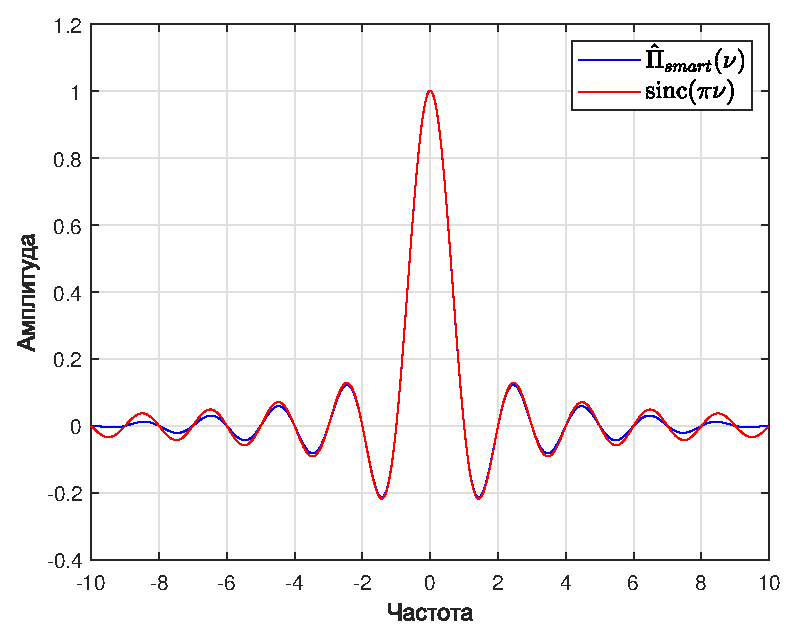
\includegraphics[width=0.55\linewidth]{graphs/3/T_50_dt_0.05005_V_20_dv_0.02/fourier_smart.eps}
    \caption{Приближение истинного Фурье-образа с использованием fft}
\end{figure}

В этом случае образ становится похож на аналитический, но чем больше модуль частоты, тем сильнее он отклоняется от аналитического, метод также действует гораздо быстрее, чем подобный ему, реализованный через функцию frapz -- в этом случае для вычисления образа функции понадобилось 0.0021 секунды.

Примем $T = 10$. Выясним влияние $\Delta t$ на график Фурье-образа функции:

\begin{figure}[H]
    \begin{minipage}{0.5\textwidth}
        \centering \includegraphics[width=\textwidth]{graphs/3/T_10_dt_0.01001_V_100_dv_0.1/fourier_smart.eps}
        \caption{$N = 1000 \Rightarrow \Delta t \approx 0.01 \Rightarrow V = 100, \Delta \nu = 0.1$}
    \end{minipage}\hfill
    \begin{minipage}{0.5\textwidth}
        \centering 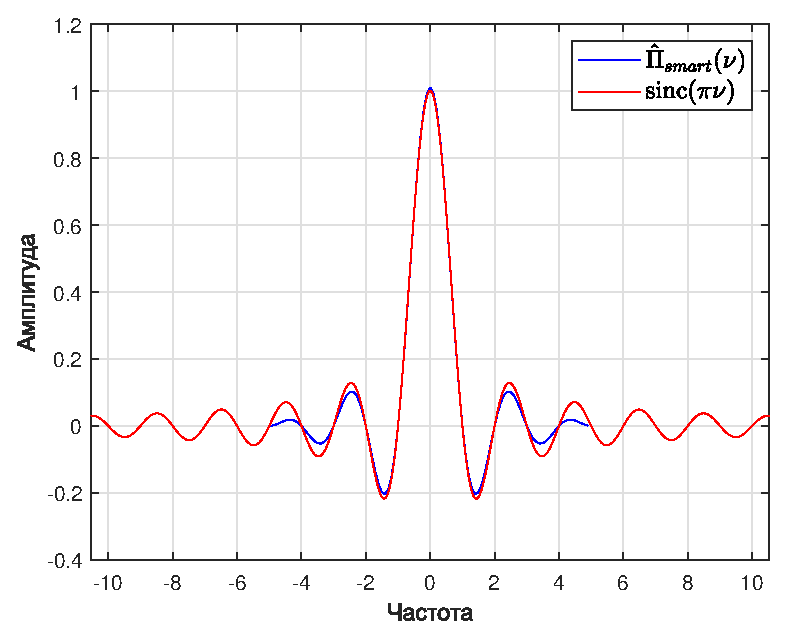
\includegraphics[width=\textwidth]{graphs/3/T_10_dt_0.10101_V_10_dv_0.1/fourier_smart.eps}
        \caption{$N = 100 \Rightarrow \Delta t \approx 0.1 \Rightarrow V = 10, \Delta \nu = 0.1$}
    \end{minipage}\\[1em]
\end{figure}\noindent\

\begin{figure}[H]
    \centering \includegraphics[width=0.55\textwidth]{graphs/3/T_10_dt_0.20408_V_5_dv_0.1/fourier_smart.eps}
    \caption{$N = 50 \Rightarrow \Delta t \approx 0.2$}
\end{figure}\noindent\

Чем больше $\Delta t$, тем меньше промежуток интегрирования  по частоте, это заметно и из графиков. Посмотрим на сравнительные графики восстановленных функций при тех же наборах значений параметров:

\begin{figure}[H]
    \begin{minipage}{0.5\textwidth}
        \centering \includegraphics[width=\textwidth]{graphs/3/T_10_dt_0.01001_V_100_dv_0.1/func_inversed_smart.eps}
        \caption{$N = 1000 \Rightarrow \Delta t \approx 0.01 \Rightarrow V = 100, \Delta \nu = 0.1$}
    \end{minipage}\hfill
    \begin{minipage}{0.5\textwidth}
        \centering \includegraphics[width=\textwidth]{graphs/3/T_10_dt_0.10101_V_10_dv_0.1/func_inversed_smart.eps}
        \caption{$N = 100 \Rightarrow \Delta t \approx 0.1 \Rightarrow V = 10, \Delta \nu = 0.1$}
    \end{minipage}\\[1em]
\end{figure}\noindent\

\begin{figure}[H]
    \centering \includegraphics[width=0.55\textwidth]{graphs/3/T_10_dt_0.20408_V_5_dv_0.1/func_inversed_smart.eps}
    \caption{$N = 50 \Rightarrow \Delta t \approx 0.2, \Delta \nu = 0.1$}
\end{figure}\noindent\

Время работы разработанного метода при всех наборах параметров примерно одинаковое -- не превышает 0.002 секунды и убывает с уменьшением $\Delta t$.

Посмотрим на то, как на графики образа влияет изменение промежутка $T$ при $\Delta t \approx 0.01$ (приблизительно равно потому что для каждого $T$ было подобрано $N$ такое, чтобы $\Delta t = \frac{T}{N-1} \approx 0.01$ с незначительной погрешностью):

\begin{figure}[H]
    \begin{minipage}{0.5\textwidth}
        \centering \includegraphics[width=\textwidth]{graphs/3/T_100_dt_0.010001_V_100_dv_0.01/fourier_smart.eps}
        \caption{$T = 1000 \Rightarrow N = 100000 \Rightarrow V = 100, \Delta \nu = 0.01$}
    \end{minipage}\hfill
    \begin{minipage}{0.5\textwidth}
        \centering \includegraphics[width=\textwidth]{graphs/3/T_50_dt_0.010002_V_100_dv_0.02/fourier_smart.eps}
        \caption{$T = 50 \Rightarrow N = 5000 \Rightarrow V = 100, \Delta \nu = 0.02$}
    \end{minipage}\\[1em]
\end{figure}\noindent\

\begin{figure}[H]
    \begin{minipage}{0.5\textwidth}
        \centering \includegraphics[width=\textwidth]{graphs/3/T_1.5_dt_0.010067_V_100_dv_0.66667/fourier_smart.eps}
        \caption{$T = 1000 \Rightarrow N = 100000 \Rightarrow V = 100, \Delta \nu = 0.01$}
    \end{minipage}\hfill
    \begin{minipage}{0.5\textwidth}
        \centering \includegraphics[width=\textwidth]{graphs/3/T_0.8_dt_0.010127_V_100_dv_1.25/fourier_smart.eps}
        \caption{$T = 50 \Rightarrow N = 5000 \Rightarrow V = 100, \Delta \nu = 0.02$}
    \end{minipage}\\[1em]
\end{figure}\noindent\

Графики восстановленной функции:

\begin{figure}[H]
    \begin{minipage}{0.5\textwidth}
        \centering \includegraphics[width=\textwidth]{graphs/3/T_100_dt_0.010001_V_100_dv_0.01/func_inversed_smart.eps}
        \caption{$T = 1000 \Rightarrow N = 100000 \Rightarrow V = 100, \Delta \nu = 0.01$}
    \end{minipage}\hfill
    \begin{minipage}{0.5\textwidth}
        \centering \includegraphics[width=\textwidth]{graphs/3/T_50_dt_0.010002_V_100_dv_0.02/func_inversed_smart.eps}
        \caption{$T = 50 \Rightarrow N = 5000 \Rightarrow V = 100, \Delta \nu = 0.02$}
    \end{minipage}\\[1em]
\end{figure}\noindent\

\begin{figure}[H]
    \begin{minipage}{0.5\textwidth}
        \centering \includegraphics[width=\textwidth]{graphs/3/T_1.5_dt_0.010067_V_100_dv_0.66667/func_inversed_smart.eps}
        \caption{$T = 1.5 \Rightarrow N = 150 \Rightarrow V = 100, \Delta \nu = \frac{2}{3}$}
    \end{minipage}\hfill
    \begin{minipage}{0.5\textwidth}
        \centering \includegraphics[width=\textwidth]{graphs/3/T_0.8_dt_0.010127_V_100_dv_1.25/func_inversed_smart.eps}
        \caption{$T = 0.8 \Rightarrow N = 80 \Rightarrow V = 100, \Delta \nu = 1.25$}
    \end{minipage}\\[1em]
\end{figure}\noindent\

Функция восстанавливается хорошо при всех рассмотренных $T$. Быстродействие не меняется в зависимости от величины $T$ -- при всех значениях параметра время выполнения метода не превысило 0.006 секунд.

\subsubsection{Сравнение действия методов}\

Сравним непрерывное преобразование, реализованное через численное интегрирование, дискретное и модификацию дискретного.

Наиболее показательные графики образов для полученных разными методами функций:

\begin{figure}[H]
    \begin{minipage}{0.5\textwidth}
        \centering \includegraphics[width=\textwidth]{graphs/3/T_5_dt_0.005005_V_200_dv_0.2/fourier_combined_all.eps}
        \caption{$T = 5, \Delta t \approx 0.005, V = 200, \Delta \nu = 0.2$} % Малое дельта т
    \end{minipage}\hfill
    \begin{minipage}{0.5\textwidth}
        \centering \includegraphics[width=\textwidth]{graphs/3/T_10_dt_0.01001_V_100_dv_0.1/fourier_combined_all.eps}
        \caption{$T = 10, \Delta t \approx 0.01, V = 100, \Delta \nu = 0.1$}
    \end{minipage}\hfill
\end{figure}\noindent\

\begin{figure}[H]
    \begin{minipage}{0.5\textwidth}
        \centering \includegraphics[width=\textwidth]{graphs/3/T_5000_dt_0.50005_V_2_dv_0.0002/fourier_combined_all.eps}
        \caption{$T = 5000, \Delta t \approx 0.5, V = 2, \Delta \nu = 0.0002$}
    \end{minipage}\hfill
    \begin{minipage}{0.5\textwidth}
        \centering \includegraphics[width=\textwidth]{graphs/3/T_0.5_dt_0.0005005_V_2000_dv_2/fourier_combined_all.eps}
        \caption{$T = 0.5, \Delta t \approx 0.0005, V = 2000, \Delta \nu = 2$}
    \end{minipage}\\[1em]
\end{figure}\noindent\

В общем случае график Фурье-образа, полученного разработанным методом, близко совпадает с графиком, полученным с помощью численного интегрирования (непрерывное преобразование), и, соответственно, с образом, полученным аналитически, кроме случая с большим $T$, из-за которого график строится на слишком маленьком промежутке $V$. В графиках восстановленных функций (обратное преобразование, примененное к полученному образу) разницы между функциями также не видно:

\begin{figure}[H]
    \begin{minipage}{0.5\textwidth}
        \centering \includegraphics[width=\textwidth]{graphs/3/T_5_dt_0.005005_V_200_dv_0.2/func_combined_all.eps}
        \caption{$T = 5, \Delta t \approx 0.005, V = 200, \Delta \nu = 0.2$} % Малое дельта т
    \end{minipage}\hfill
    \begin{minipage}{0.5\textwidth}
        \centering \includegraphics[width=\textwidth]{graphs/3/T_10_dt_0.01001_V_100_dv_0.1/func_combined_all.eps}
        \caption{$T = 10, \Delta t \approx 0.01, V = 100, \Delta \nu = 0.1$}
    \end{minipage}\hfill
\end{figure}\noindent\

\begin{figure}[H]
    \begin{minipage}{0.5\textwidth}
        \centering \includegraphics[width=\textwidth]{graphs/3/T_5000_dt_0.50005_V_2_dv_0.0002/func_combined_all.eps}
        \caption{$T = 5000, \Delta t \approx 0.5, V = 2, \Delta \nu = 0.0002$}
    \end{minipage}\hfill
    \begin{minipage}{0.5\textwidth}
        \centering \includegraphics[width=\textwidth]{graphs/3/T_0.5_dt_0.0005005_V_2000_dv_2/func_combined_all.eps}
        \caption{$T = 0.5, \Delta t \approx 0.0005, V = 2000, \Delta \nu = 2$}
    \end{minipage}\\[1em]
\end{figure}\noindent\

Точность метода в сравнении с ранее реализованными остаётся высокой, почти неотличимой (если не рассматривать графики образов -- очевидно, дискретное преобразование возвращает иной образ), также не удалось найти значения $T$ и $\Delta t$, при которых метод будет проигрывать численному интегрированию или DFT.
Модифицированный FFT работает примерно в 3 раза дольше, чем обычный, однако разница с численным интегрированием огромна. Среднее время для всех найденных численным интегрированием образов составляет 0.71 секунд, при нахождении образа через FFT -- 0.00077, а для модифицированного FFT -- 0.0021.

\subsubsection{Выводы}\

В реализованном методе количество значений индекса $m$ должно совпадать с количеством значений индекса $n$, а это накладывает ограничение на выбор $V$ и $\Delta \nu$ при выбранных $T$ и $\Delta t$ -- должно выполняться равенство $V / \Delta \nu = T/\Delta t, V = len([-B, B])$, где $[-B, B]$ -- промежуток интегрирования по частоте. Притом для того, чтобы получаемый образ совпадал с аналитическим, необходимо выполнение $B = N/2T$. Из-за этого условия увеличение $T$ влечет за собой уменьшение $V$, и приводит к увеличению $\Delta \nu$, увеличение $\Delta t$ же влияет ровно противоположным образом. Быстродействие метода обусловливается его низкой в сравнении с численным интегрированием вычислительной сложностью -- $O(N \cdot log(N))$, что совпадает с вычислительной сложностью стандартного $FFT$, но вычислений на каждом шаге больше, что делает его более затратным, и выполняется он дольше.

\section{Сэмплирование}\

Примем параметры $a_1 = a_2 = \omega_1 = \omega_2 = \varphi_1 = \varphi_2 = b = 1$.


\subsection{Первая функция}

Рассмотрим функцию

$$
y_1(t) = a_1\sin{(\omega_1t + \varphi_1)} + a_2\sin{(\omega_2t+\varphi_2)}.
$$\ 

Её график на промежутке длиной $T = 10$ с количеством входящих в промежуток точек $N = 1000$:

\begin{figure}[H]
    \centering
    \includegraphics[width=0.5\linewidth]{graphs2/func1.eps}
    \caption{$y_1(t) = \sin{(t + 1)} + \sin{(t+1)}$}
\end{figure}

Проведем сэмплирование функции с $T = 50, \Delta t = 0.1$, вот получившийся сравнительный график исходной и сэмплированной функций:

\begin{figure}[H]
    \centering
    \includegraphics[width=0.5\linewidth]{graphs2/func1+discrete.eps}
    \caption{$y_1(t_n) = \sin{(t + 1)} + \sin{(t+1)}$}
\end{figure}

Попробуем применить интерполяционную формулу $y_1(t_n) = \sum_{n=-B}^{B} y_1(t_n) \cdot \operatorname{sinc}(2B(t-t_n))$ к сэмплированному варианту функции при $B = \frac{1}{2\Delta t} = 5, \Delta \nu = \frac{1}{T}=0.02$ -- вот получившийся график:

\begin{figure}[H]
    \centering
    \includegraphics[width=0.5\linewidth]{graphs2/func1_recovered.eps}
    \caption{$y_1(t_n) = \sin{(t + 1)} + \sin{(t+1)}$}
\end{figure}

Видим, что при таких наборах параметров исходная функция восстановилась полностью, посмотрим на получающуюся функцию при других значениях этих параметров. 

Посмотрим, как меняется восстановленная функция при изменении $\Delta t$ при фиксированном $T$. При $T = 50 \Rightarrow \Delta \nu = 0.02$ ($B=\frac{1}{2\Delta t}$):

\begin{figure}[H]
    \begin{minipage}{0.5\textwidth}
        \centering \includegraphics[width=\textwidth]{graphs2/T_50_dt_0.5_B_1_dv_0.02/func1_recovered.eps}
        \caption{$\Delta t = 0.5 \Rightarrow B = 1$}
    \end{minipage}\hfill
    \begin{minipage}{0.5\textwidth}
        \centering \includegraphics[width=\textwidth]{graphs2/T_50_dt_1_B_0.5_dv_0.02/func1_recovered.eps}
        \caption{$\Delta t = 1 \Rightarrow B = 0.5$}
    \end{minipage}\\[1em]
\end{figure}\noindent\

\begin{figure}[H]
    \begin{minipage}{0.5\textwidth}
        \centering \includegraphics[width=\textwidth]{graphs2/T_50_dt_2_B_0.25_dv_0.02/func1_recovered.eps}
        \caption{$\Delta t = 2 \Rightarrow B = 0.25$}
    \end{minipage}\hfill
    \begin{minipage}{0.5\textwidth}
        \centering \includegraphics[width=\textwidth]{graphs2/T_50_dt_3_B_0.16667_dv_0.02/func1_recovered.eps}
        \caption{$\Delta t = 3 \Rightarrow B = 1/6$}
    \end{minipage}\\[1em]
\end{figure}\noindent\

\begin{figure}[H]
    \centering
    \includegraphics[width=0.55\linewidth]{graphs2/T_50_dt_5_B_0.1_dv_0.02/func1_recovered.eps}
    \caption{$\Delta t = 5 \Rightarrow B = 0.1$}
\end{figure}

Видим, что при $\Delta t > 2$ функция уже не восстанавливается должным образом.

Графики образов, полученных реализованным в пункте 1.4 методом, для рассмотренных наборов значений параметров ($T = 50 \Rightarrow \Delta \nu = 0.02$):

\begin{figure}[H]
    \begin{minipage}{0.5\textwidth}
        \centering \includegraphics[width=\textwidth]{graphs2/T_50_dt_0.5_B_1_dv_0.02/func1_image.eps}
        \caption{$\Delta t = 0.5 \Rightarrow B = 1$}
    \end{minipage}\hfill
    \begin{minipage}{0.5\textwidth}
        \centering \includegraphics[width=\textwidth]{graphs2/T_50_dt_1_B_0.5_dv_0.02/func1_image.eps}
        \caption{$\Delta t = 1 \Rightarrow B = 0.5$}
    \end{minipage}\\[1em]
\end{figure}\noindent\

\begin{figure}[H]
    \begin{minipage}{0.5\textwidth}
        \centering \includegraphics[width=\textwidth]{graphs2/T_50_dt_2_B_0.25_dv_0.02/func1_image.eps}
        \caption{$\Delta t = 2 \Rightarrow B = 0.25$}
    \end{minipage}\hfill
    \begin{minipage}{0.5\textwidth}
        \centering \includegraphics[width=\textwidth]{graphs2/T_50_dt_3_B_0.16667_dv_0.02/func1_image.eps}
        \caption{$\Delta t = 3 \Rightarrow B = 1/6$}
    \end{minipage}\\[1em]
\end{figure}\noindent\

\begin{figure}[H]
    \centering
    \includegraphics[width=0.55\linewidth]{graphs2/T_50_dt_5_B_0.1_dv_0.02/func1_image.eps}
    \caption{$\Delta t = 5 \Rightarrow B = 0.1$}
\end{figure}

Рассмотрим влияние $T$, зафиксируем $\Delta t = 0.5 \Rightarrow B = 1$, получим следующие графики:

\begin{figure}[H]
    \begin{minipage}{0.5\textwidth}
        \centering \includegraphics[width=\textwidth]{graphs2/T_2_dt_0.5_B_1_dv_0.5/func1_recovered.eps}
        \caption{$T = 2 \Rightarrow \Delta \nu = 0.5$}
    \end{minipage}\hfill
    \begin{minipage}{0.5\textwidth}
        \centering \includegraphics[width=\textwidth]{graphs2/T_4_dt_0.5_B_1_dv_0.25/func1_recovered.eps}
        \caption{$T = 4 \Rightarrow \Delta \nu = 0.25$}
    \end{minipage}\\[1em]
\end{figure}\noindent\

\begin{figure}[H]
    \begin{minipage}{0.5\textwidth}
        \centering \includegraphics[width=\textwidth]{graphs2/T_10_dt_0.5_B_1_dv_0.1/func1_recovered.eps}
        \caption{$T = 10 \Rightarrow \Delta \nu = 0.1$}
    \end{minipage}\hfill
    \begin{minipage}{0.5\textwidth}
        \centering \includegraphics[width=\textwidth]{graphs2/T_25_dt_0.5_B_1_dv_0.04/func1_recovered.eps}
        \caption{$T = 25 \Rightarrow \Delta \nu = 0.04$}
    \end{minipage}\\[1em]
\end{figure}\noindent\

При увеличении $T$ уменьшается шаг интегрирования по частоте, и функция восстанавливается лучше.

Посмотрим, как ведут себя образы функций на рассмотренных наборах значений параметров:

\begin{figure}[H]
    \begin{minipage}{0.5\textwidth}
        \centering \includegraphics[width=\textwidth]{graphs2/T_2_dt_0.5_B_1_dv_0.5/func1_image.eps}
        \caption{$T = 2 \Rightarrow \Delta \nu = 0.5$}
    \end{minipage}\hfill
    \begin{minipage}{0.5\textwidth}
        \centering \includegraphics[width=\textwidth]{graphs2/T_4_dt_0.5_B_1_dv_0.25/func1_image.eps}
        \caption{$T = 4 \Rightarrow \Delta \nu = 0.25$}
    \end{minipage}\\[1em]
\end{figure}\noindent\

\begin{figure}[H]
    \begin{minipage}{0.5\textwidth}
        \centering \includegraphics[width=\textwidth]{graphs2/T_10_dt_0.5_B_1_dv_0.1/func1_image.eps}
        \caption{$T = 10 \Rightarrow \Delta \nu = 0.1$}
    \end{minipage}\hfill
    \begin{minipage}{0.5\textwidth}
        \centering \includegraphics[width=\textwidth]{graphs2/T_25_dt_0.5_B_1_dv_0.04/func1_image.eps}
        \caption{$T = 25 \Rightarrow \Delta \nu = 0.04$}
    \end{minipage}\\[1em]
\end{figure}\noindent\

С увеличением рассматриваемого промежутка уменьшается шаг по частоте, и становится более отчетливым пик, указывающий на синусоидальность исходного сигнала.

\subsection{Вторая функция}

Теперь рассмотрим функцию $y_2(t) = \operatorname{sinc}(bt)$, значение параметра $b = 1$ уже было выбрано ранее, рассмотрим график полученной функции $y_2(t) = \operatorname{sinc}(t)$:

\begin{figure}[H]
    \centering
    \includegraphics[width=0.55\linewidth]{graphs2/func2.eps}
    \caption{$y_2(t) = \operatorname{sinc}(t)$}
\end{figure}\ 

Видим, что, в отличие от предыдущей рассматриваемой функции, эта не является периодической. Сравнительный график с сэмплированным вариантом:

\begin{figure}[H]
    \centering
    \includegraphics[width=0.55\linewidth]{graphs2/func2+discrete.eps}
    \caption{$y_2(t_n) = \operatorname{sinc}(t_n)$}
\end{figure}\ 

Восстановим функцию из её сэмплированного вида при помощи интерполяционной формулы:

\begin{figure}[H]
    \centering
    \includegraphics[width=0.55\linewidth]{graphs2/func2_recovered.eps}
    \caption{Результат применения интерполяционной формулы к $\operatorname{sinc}(t_n)$}
\end{figure}\ 

Видим, что функция полностью восстановилась. Посмотрим на график образа для получившейся функции, ее сэмплированного варианта и оригинала:

\begin{figure}[H]
    \centering
    \includegraphics[width=0.55\linewidth]{graphs2/func2_image.eps}
    \caption{$y_2(t_n) = \operatorname{sinc}(t_n)$}
\end{figure}\

Как и ожидалось, результат похож на аналитически найденный в прошлых лабораторных образ -- на прямоугольную функцию. Исследуем влияние значения параметра $\Delta t$ на способность интерполяционной формулы восстанавливать функцию при фиксированном $T = 50 \Rightarrow \Delta \nu = 0.02$:

\begin{figure}[H]
    \begin{minipage}{0.5\textwidth}
        \centering \includegraphics[width=\textwidth]{graphs2/T_50_dt_0.5_B_1_dv_0.02/func2_recovered.eps}
        \caption{$\Delta t = 0.5 \Rightarrow B = 1$}
    \end{minipage}\hfill
    \begin{minipage}{0.5\textwidth}
        \centering \includegraphics[width=\textwidth]{graphs2/T_50_dt_1_B_0.5_dv_0.02/func2_recovered.eps}
        \caption{$\Delta t = 1 \Rightarrow B = 0.5$}
    \end{minipage}\\[1em]
\end{figure}\noindent\

\begin{figure}[H]
    \begin{minipage}{0.5\textwidth}
        \centering \includegraphics[width=\textwidth]{graphs2/T_50_dt_2_B_0.25_dv_0.02/func2_recovered.eps}
        \caption{$\Delta t = 2 \Rightarrow B = 0.25$}
    \end{minipage}\hfill
    \begin{minipage}{0.5\textwidth}
        \centering \includegraphics[width=\textwidth]{graphs2/T_50_dt_3_B_0.16667_dv_0.02/func2_recovered.eps}
        \caption{$\Delta t = 3 \Rightarrow B = 1/6$}
    \end{minipage}\\[1em]
\end{figure}\noindent\

В этом случае, в отличие от предыдущего варианта с линейной комбинацией синусов, функция перестала восстанавливаться с высокой точностью гораздо раньше -- значительное отклонение от оригинальной функции наблюдается уже при $\Delta t = 1$, а при $\Delta t = 3$ почти полностью теряет изначальный вид.

Сравнительные графики образов получившихся функций:

\begin{figure}[H]
    \begin{minipage}{0.5\textwidth}
        \centering \includegraphics[width=\textwidth]{graphs2/T_50_dt_0.5_B_1_dv_0.02/func2_image.eps}
        \caption{$\Delta t = 0.5 \Rightarrow B = 1$}
    \end{minipage}\hfill
    \begin{minipage}{0.5\textwidth}
        \centering \includegraphics[width=\textwidth]{graphs2/T_50_dt_1_B_0.5_dv_0.02/func2_image.eps}
        \caption{$\Delta t = 1 \Rightarrow B = 0.5$}
    \end{minipage}\\[1em]
\end{figure}\noindent\

\begin{figure}[H]
    \begin{minipage}{0.5\textwidth}
        \centering \includegraphics[width=\textwidth]{graphs2/T_50_dt_2_B_0.25_dv_0.02/func2_image.eps}
        \caption{$\Delta t = 2 \Rightarrow B = 0.25$}
    \end{minipage}\hfill
    \begin{minipage}{0.5\textwidth}
        \centering \includegraphics[width=\textwidth]{graphs2/T_50_dt_3_B_0.16667_dv_0.02/func2_image.eps}
        \caption{$\Delta t = 3 \Rightarrow B = 1/6$}
    \end{minipage}\\[1em]
\end{figure}\noindent\

Фурье-образы при увеличении $\Delta t$ также теряют свой первоначальный облик, при малых значениях $\Delta t$ начинают походить на ``реальный'' образ (прямоугольную функцию).

Зафиксируем $\Delta t = 0.5 \Rightarrow B = 1$ и посмотрим, как на восстановление исходной функции при помощи формулы интерполяции влияет значение $T$:

\begin{figure}[H]
    \begin{minipage}{0.5\textwidth}
        \centering \includegraphics[width=\textwidth]{graphs2/T_2_dt_0.5_B_1_dv_0.5/func2_recovered.eps}
        \caption{$T = 2 \Rightarrow \Delta \nu = 0.5$}
    \end{minipage}\hfill
    \begin{minipage}{0.5\textwidth}
        \centering \includegraphics[width=\textwidth]{graphs2/T_25_dt_0.5_B_1_dv_0.04/func2_recovered.eps}
        \caption{$T = 4 \Rightarrow \Delta \nu = 0.25$}
    \end{minipage}\\[1em]
\end{figure}\noindent\

\begin{figure}[H]
    \begin{minipage}{0.5\textwidth}
        \centering \includegraphics[width=\textwidth]{graphs2/T_200_dt_0.5_B_1_dv_0.005/func2_recovered.eps}
        \caption{$T = 200 \Rightarrow \Delta \nu = 0.005$}
    \end{minipage}\hfill
    \begin{minipage}{0.5\textwidth}
        \centering \includegraphics[width=\textwidth]{graphs2/T_1000_dt_0.5_B_1_dv_0.001/func2_recovered.eps}
        \caption{$T = 1000 \Rightarrow \Delta \nu = 0.001$}
    \end{minipage}\\[1em]
\end{figure}\noindent\

Почему-то при $T = 1000$ восстановленная функция стала плохо походить на исходную. Чтобы понять, почему это произошло, построим сравнительные графики Фурье-образов получившихся функций:

\begin{figure}[H]
    \begin{minipage}{0.5\textwidth}
        \centering \includegraphics[width=\textwidth]{graphs2/T_2_dt_0.5_B_1_dv_0.5/func2_image.eps}
        \caption{$T = 2 \Rightarrow \Delta \nu = 0.5$}
    \end{minipage}\hfill
    \begin{minipage}{0.5\textwidth}
        \centering \includegraphics[width=\textwidth]{graphs2/T_25_dt_0.5_B_1_dv_0.04/func2_image.eps}
        \caption{$T = 4 \Rightarrow \Delta \nu = 0.25$}
    \end{minipage}\\[1em]
\end{figure}\noindent\

\begin{figure}[H]
    \begin{minipage}{0.5\textwidth}
        \centering \includegraphics[width=\textwidth]{graphs2/T_200_dt_0.5_B_1_dv_0.005/func2_image.eps}
        \caption{$T = 200 \Rightarrow \Delta \nu = 0.005$}
    \end{minipage}\hfill
    \begin{minipage}{0.5\textwidth}
        \centering \includegraphics[width=\textwidth]{graphs2/T_1000_dt_0.5_B_1_dv_0.001/func2_image.eps}
        \caption{$T = 1000 \Rightarrow \Delta \nu = 0.001$}
    \end{minipage}\\[1em]
\end{figure}\noindent\

Заметно, что увеличение промежутка интегрирования по времени влечет за собой увеличение точности образа восстанавливаемой функции, однако чересчур большое значение $T$ приводит к выходу значимой части образа за промежуток $[-B, B]$, что негативно сказывается на точности восстановленной функции.

\subsection{Выводы}\

Интерполяционная формула менее чувствительна к изменениям $\Delta t$ и $T$ в случае с первой функцией, это связано с её периодичностью. Выявлено, что при $\Delta t = 1/(2B)$ функция может быть безошибочно восстановлена из своего сэмплированного представления при достаточно больших $N$, что подтверждает выполнение теоремы Найквиста-Шеннона-Котельникова.

\section{Вывод}\

В ходе выполнения работы была сравнена точность и быстродействие реализаций непрерывного и дискретного преобразование Фурье, разработан метод для приближения к реальному (найденному аналитически) образу при помощи быстрого преобразования Фурье, выявлена связь между непрерывным и периодическим, проведено сэмплирование и подтверждено выполнение одной из главных теорем в теории сигналов, позволяющей безошибочно восстанавливать непрерывный сигнал из дискретного.

\newpage

\section{Приложение А. Код для выполнения заданий}

\subsection*{Листинг 1. Код для выполнения пункта 1.1}

\begin{lstlisting}[caption={Код для построения графиков для пункта 1.1}, language=matlab]
t = 10;
T = [-t/2, t/2];
dt = 0.5;
a = min(T);
b = max(T);

v = 12;
V = [-v/2, v/2];
dv = 0.001;
v0 = min(V);
v1 = max(V);

parametres = "T_" + num2str(t) + "_dt_" + num2str(dt) + "_V_" + num2str(v) + "_dv_"+ num2str(dv);
path = "FM-LAB5" + filesep + parametres + filesep;
if ~exist(path, 'dir')
    mkdir(path);
end

t = linspace(a, b, (1/dt)*t);
nu = linspace(v0, v1, (1/dv)*v);
nu_static = linspace(v0, v1, 1000);
t_static = linspace(a, b, 1000);

Pi_t = abs(t) <= 0.5;
Pi_t_static = abs(t_static) <= 0.5;
Pi_nu = sinc(nu_static);

Pi_nu_numerical = zeros(size(nu));
tic
for k = 1:length(nu)
    integrand = Pi_t .* exp(-1j * 2 * pi * nu(k) * t);
    Pi_nu_numerical(k) = trapz(t, integrand);
end
toc

Pi_t_inversed = zeros(size(t));

for k = 1:length(t)
    integrand = Pi_nu_numerical .* exp(1j * 2 * pi * nu * t(k));
    Pi_t_inversed(k) = trapz(nu, integrand);
end

p_fourier_numerical = figure;
plot(nu, Pi_nu_numerical, 'Color', 'b');
hold on;
plot(nu_static, Pi_nu, 'Color', 'r');
xlabel('Частота');
ylabel('Амплитуда');
real_Pi_num = real(Pi_nu_numerical);
ylim([-(abs(min(real_Pi_num))+abs(min(real_Pi_num))*0.2), max(real_Pi_num)+max(real_Pi_num)*0.2])
xlim([max(-10, min(nu)), min(10, max(nu))])
legend('$\hat{\Pi}(\nu)$', '$\mathrm{sinc}(\pi\nu)$', 'Interpreter', 'latex', 'fontsize', 11)
grid on;
legend(BackgroundAlpha=.6);
saveas(p_fourier_numerical, path + "fourier_numerical.png", "png")

p_t_inversed_numerical = figure;
plot(t, Pi_t_inversed, 'Color', 'b');
hold on;
plot(t_static, Pi_t_static, 'Color', 'black');
xlabel('t');
ylabel('\Pi(t)');
% ylim([min(Pi_t_inversed)+min(Pi_t_inversed)*0.2, max(Pi_t_inversed)+max(Pi_t_inversed)*0.2])
xlim([-3, 3]);
xticks(-5:1:5);
legend('$\mathcal{F}^{-1}\{\hat{\Pi}(\nu)\}$', '$\Pi(t)$', 'Interpreter', 'latex', 'fontsize', 11)
grid on;
legend(BackgroundAlpha=.6);
saveas(p_t_inversed_numerical, path+"func_inversed_fourier.png", "png")
\end{lstlisting}

\subsection*{Листинг 2. Код для выполнения пункта 1.2}

\begin{lstlisting}[caption={Код для построения графиков для пункта 1.2}, language=matlab]
t = 2;
T = [-t/2, t/2];
dt = 0.01;
a = min(T);
b = max(T);

v = 1/dt;
V = [-v/2, v/2];
dv = 1/t;
v0 = min(V);
v1 = max(V);

parametres = "T_" + num2str(t) + "_dt_" + num2str(dt) + "_V_" + num2str(v) + "_dv_"+ num2str(dv);
path = "FM-LAB5" + filesep + parametres + filesep;
if ~exist(path, 'dir')
    mkdir(path);
end

t = linspace(a, b, (1/dt)*t);
N = length(t);
nu = linspace(v0, v1, (1/dv)*v);
nu_static = linspace(v0, v1, 10000);
t_static = linspace(a, b, 10000);

Pi_t = abs(t) <= 0.5;
Pi_t_static = abs(t_static) <= 0.5;
Pi_nu = sinc(nu_static);

tic
Pi_nu_numerical = fftshift(fft(Pi_t)) / sqrt(N);
toc
Pi_t_inversed = ifft(ifftshift(Pi_nu_numerical)) * sqrt(N);

p_fourier_numerical = figure;
plot(nu, Pi_nu_numerical, 'Color', 'b');
hold on;
plot(nu_static, Pi_nu, 'Color', 'r');
xlabel('Частота');
ylabel('Амплитуда');
real_Pi_num = real(Pi_nu_numerical);
% ylim([-(abs(min(real_Pi_num))+abs(min(real_Pi_num))*0.2), max(real_Pi_num)+max(real_Pi_num)*0.2])
xlim([max(-10, min(nu)), min(10, max(nu))])
legend('$\hat{\Pi}(\nu)$', '$\mathrm{sinc}(\pi\nu)$', 'Interpreter', 'latex', 'fontsize', 11)
grid on;
legend(BackgroundAlpha=.6);
saveas(p_fourier_numerical, path + "fourier_numerical.png", "png")

p_t_inversed_numerical = figure;
plot(t, Pi_t_inversed, 'Color', 'b');
hold on;
plot(t_static, Pi_t_static, 'Color', 'black');
xlabel('t');
ylabel('\Pi(t)');
ylim([-0.2, 1.2]);
xlim([-3, 3]);
xticks(-5:1:5);
legend('$\mathcal{F}^{-1}\{\hat{\Pi}(\nu)\}$', '$\Pi(t)$', 'Interpreter', 'latex', 'fontsize', 11)
grid on;
legend(BackgroundAlpha=.6);
saveas(p_t_inversed_numerical, path+"func_inversed_fourier.png", "png")
\end{lstlisting}

\subsection*{Листинг 3. Код для выполнения пункта 1.4}

\begin{lstlisting}[caption={Код для построения графиков для пункта 1.3}, language=matlab]
T = 5000;
N = 10000;
a = -T/2;
b = T/2;
delta_t = T/(N-1);
B = N/2;  % Образ Фурье содержится внутри отрезка [-B, B-1], B = N/2T, и при остальных не сходится с реальным образом

n = linspace(0, N-1, N);
t_n = a + n * delta_t;

parametres = "T_" + num2str(T) + "_dt_" + num2str(delta_t) + "_V_" + num2str((B*2)/T) + "_dv_" + num2str((B*2)/(T*N));
path = "FM-LAB5" + filesep + parametres + filesep;
if ~exist(path, 'dir')
    mkdir(path);
end
Pi_t = abs(t_n) <= 0.5;
t_n_static = linspace(-10, 10, 10000);
Pi_t_static = abs(t_n_static) <= 0.5;

m = linspace(0, N-1, N);
start = tic;
c_m = delta_t * exp(1i * pi * m);
rect_image_smart = fftshift(c_m.*fft(Pi_t));
time_inversed_smart = toc(start);
rect_inversed_smart = ifft(ifftshift(rect_image_smart)./c_m);

v_m = linspace(-B, B-1, N) / T;
v_static = linspace(-100, 100, 10000);
rect_v_static = sinc(v_static);

p_image_smart = figure;
plot(v_m, real(rect_image_smart), 'Color', 'b');
hold on;
plot(v_static, sinc(v_static), 'Color', 'r');
eps = 0.03;
xmax = max(v_static(rect_v_static > eps));
xlim([-xmax, xmax]);
% xlim([-1.5, 1.5]);
xlabel('Частота');
ylabel('Амплитуда');
legend('$\hat{\Pi}_{smart}(\nu)$', '$\mathrm{sinc}(\pi\nu)$', 'Interpreter', 'latex', 'fontsize', 12)
grid on;
legend(BackgroundAlpha=.6);
exportgraphics(p_image_smart, path + "fourier_smart.eps")

p_inv_smart = figure;
plot(t_n, real(rect_inversed_smart), 'Color', 'b');
hold on;
plot(t_n_static, Pi_t_static, 'Color', 'black');
xlabel('t');
ylabel('\Pi(t)');
xlim([-3, 3]);
ylim([-0.2, 1.2]);
xticks(-5:1:5);
legend('$\mathcal{F}^{-1}\{\hat{\Pi}_{smart}(\nu)\}$', '$\Pi(t)$', 'Interpreter', 'latex', 'fontsize', 12)
grid on;
legend(BackgroundAlpha=.6);
exportgraphics(p_inv_smart, path+"func_inversed_smart.eps")

% % % % % % % % % % % % % % % % % % % % % % % % % % % % % % % % % % % % % %

start = tic; %
rect_image_dft = fftshift(fft(Pi_t)) / sqrt(N);
rect_image_time = toc(start); %
rect_inversed_dft = ifft(ifftshift(rect_image_dft)) * sqrt(N);

rect_image_numerical = zeros(size(v_m));


start = tic;
for k = 1:length(v_m)
    integrand = Pi_t .* exp(-1j * 2 * pi * v_m(k) * t_n);
    rect_image_numerical(k) = trapz(t_n, integrand);
end
rect_image_numerical_time = toc(start);

rect_inversed_numerical = zeros(size(t_n));

for k = 1:length(t_n)
    integrand = rect_image_numerical .* exp(1j * 2 * pi * v_m * t_n(k));
    rect_inversed_numerical(k) = trapz(v_m, integrand);
end

p_fourier_combined_all = figure;
plot(v_m, real(rect_image_dft), 'Color', 'r');
hold on;
plot(v_m, real(rect_image_smart), 'Color', 'b');
plot(v_m, real(rect_image_numerical), 'Color', 'g');
plot(v_static, rect_v_static, 'Color', 'black');
% xlim([-1.5, 1.5]);
xlabel('Частота');
ylabel('Амплитуда');
eps = 0.05;
xmax = max(v_static(rect_v_static > eps));
xlim([-xmax, xmax]);
ylim([min(rect_v_static), max(rect_v_static)]);
legend('$\hat{\Pi}_{DFT}(\nu)$', '$\hat{\Pi}_{smart}(\nu)$', '$\hat{\Pi}_{numerical}(\nu)$', '$\mathrm{sinc}(\pi\nu)$', 'Interpreter', 'latex', 'fontsize', 12)
grid on;
legend(BackgroundAlpha=.6);
exportgraphics(p_fourier_combined_all, path + "fourier_combined_all.eps")

p_func_combined_all = figure;
plot(t_n, rect_inversed_dft, 'Color', 'r');
hold on;
plot(t_n, rect_inversed_smart, 'Color', 'b');
plot(t_n, real(rect_inversed_numerical), 'Color', 'g');
plot(t_n_static, Pi_t_static, 'Color', 'black');
% eps = 0.1;
% xmax = max(t_n_static(Pi_t_static > eps));
% xlim([-xmax, xmax]);
xlim([-3, 3]);
ylim([-0.2, 1.2]);
xlabel('Частота');
ylabel('Амплитуда');
real_Pi_num = real(rect_image_smart);
legend('$\Pi_{DFT}(t)$', '$\Pi_{smart}(t)$', '$\Pi_{numerical}(t)$', '$\Pi(t)$', 'Interpreter', 'latex', 'fontsize', 12)
grid on;
legend(BackgroundAlpha=.6);
exportgraphics(p_func_combined_all, path + "func_combined_all.eps")

f = fopen(path + num2str(time_inversed_smart) + "_" + num2str(rect_image_time) + "_" + num2str(rect_image_numerical_time), 'w' );  
fclose(f);
\end{lstlisting}

\subsection*{Листинг 4. Код для выполнения пунктов 2.1, 2.2}

\begin{lstlisting}[caption={Код для построения графиков для пунктов 2.1, 2.2}, language=matlab]
a1 = 1;
a2 = 1;
w1 = 1;
w2 = 1;
phi1 = 1;
phi2 = 1;
b = 1;

B = 1;
dt = 1/(3*B);
t1 = -100;
t2 = 100;
T = t2-t1;
N = 1000;
dv = 1 / T;
dv_n = 1 / T;
parametres = "T_" + num2str(T) + "_dt_" + num2str(dt) + "_B_" + num2str(B) + "_dv_" + num2str(dv);
path = "FM-LAB5" + filesep + parametres + filesep;
if ~exist(path, 'dir')
    mkdir(path);
end

t = linspace(t1, t2, N);
t_static = linspace(t1, t2, T*100);
t_n = linspace(t1, t2, T/dt);

y1 = a1 * sin(w1 * t + phi1) + a2 * sin(w1 * t + phi2);
y2 = sinc(b * t);

y1_static = a1 * sin(w1 * t_static + phi1) + a2 * sin(w1 * t_static + phi2);
y2_static = sinc(b * t_static);

y1_n = a1 * sin(w1 * t_n + phi1) + a2 * sin(w1 * t_n + phi2);
y2_n = sinc(b * t_n);

y_interp1 = zeros(size(t));
y_interp2 = zeros(size(t));
for i = 1:length(t)
    for n = 1:length(t_n)
        y_interp1(i) = y_interp1(i) + y1_n(n) * sinc(2 * B * (t(i) - t_n(n)));
        y_interp2(i) = y_interp2(i) + y2_n(n) * sinc(2 * B * (t(i) - t_n(n)));
    end
end

N_n = T/dt;
c_m = dt * exp(1i * pi * linspace(0, N-1, N));
c_m_n = dt * exp(1i * pi * linspace(0, N_n-1, N_n));
v_m = linspace(-B, B, N);
v_m_n = linspace(-B, B, N_n);

func1_image = fftshift(c_m.*fft(y1)) / sqrt(N);
func2_image = fftshift(c_m.*fft(y2)) / sqrt(N);

sample1_image = fftshift(c_m_n.*fft(y1_n)) / sqrt(N_n);
sample2_image = fftshift(c_m_n.*fft(y2_n)) / sqrt(N_n);

interp1_image = fftshift(c_m.*fft(y_interp1)) / sqrt(N);
interp2_image = fftshift(c_m.*fft(y_interp2)) / sqrt(N);

p_image1 = figure;
plot(v_m, func1_image, 'Color', 'black')
hold on;
plot(v_m, interp1_image, 'Color', 'g')
plot(v_m_n, sample1_image, 'Color', 'r')
line([-B, -B], ylim, 'Color', 'black')
line([B, B], ylim, 'Color', 'black')
% eps = 0.002;
% xmax = max(v_m_n(sample1_image > eps));
xlim([-B - B/10, B + B / 10]);
xlabel('Частота');
ylabel('Амплитуда');
% xlim([t1/5, t2/5]);
legend('$\hat{y}_1(\nu)$', '$\hat{y}_{1_{recovered}}(\nu)$', '$\hat{y}_1(\nu_n)$', 'Interpreter', 'latex', 'fontsize', 12)
grid on;
legend(BackgroundAlpha=.6);
exportgraphics(p_image1, path+"func1_image.eps")

p_image2 = figure;
plot(v_m, func2_image, 'Color', 'black')
hold on;
plot(v_m, interp2_image, 'Color', 'g')
plot(v_m_n, sample2_image, 'Color', 'r')
line([-B, -B], ylim, 'Color', 'black')
line([B, B], ylim, 'Color', 'black')
xlim([-B - B/10, B + B / 10]);
% eps = 0.0001;
% xmax = max(v_m_n(sample2_image > eps));
% xlim([-xmax, xmax]);
xlabel('Частота');
ylabel('Амплитуда');
% xlim([t1/5, t2/5]);
legend('$\hat{y}_2(\nu)$', '$\hat{y}_{2_{recovered}}(\nu)$', '$\hat{y}_2(\nu_n)$', 'Interpreter', 'latex', 'fontsize', 12)
grid on;
legend(BackgroundAlpha=.6);
exportgraphics(p_image2, path+"func2_image.eps")

p1 = figure;
plot(t_static, y1_static, 'Color', 'black')
xlabel('t');
ylabel('y(t)');
xlim([-5, 5]);
legend('$y_1(t)$', 'Interpreter', 'latex', 'fontsize', 12)
grid on;
legend(BackgroundAlpha=.6);
exportgraphics(p1, path+"func1.eps")

p2 = figure;
plot(t_static, y2_static, 'Color', 'black')
xlabel('t');
ylabel('y(t)');
xlim([-5, 5]);
legend('$y_2(t)$', 'Interpreter', 'latex', 'fontsize', 12)
grid on;
legend(BackgroundAlpha=.6);
exportgraphics(p2, path+"func2.eps")

p1n = figure;
plot(t_static, y1_static, 'Color', 'black')
hold on;
plot(t_n, y1_n, '.', 'Color', 'red', 'MarkerSize', 9)
xlabel('t');
ylabel('y(t)');
xlim([-5, 5]);
legend('$y_1(t)$', '$y_1(t_n)$', 'Interpreter', 'latex', 'fontsize', 12)
grid on;
legend(BackgroundAlpha=.6);
exportgraphics(p1n, path+"func1+discrete.eps")

p2n = figure;
plot(t_static, y2_static, 'Color', 'black')
hold on;
plot(t_n, y2_n, '.', 'Color', 'red', 'MarkerSize', 9)
xlabel('t');
ylabel('y(t)');
xlim([-5, 5]);
legend('$y_2(t)$', '$y_2(t_n)$', 'Interpreter', 'latex', 'fontsize', 12)
grid on;
legend(BackgroundAlpha=.6);
exportgraphics(p2n, path+"func2+discrete.eps")

p_rebuilt1 = figure;
plot(t_static, y1_static, 'Color', 'black')
hold on;
plot(t, y_interp1, 'Color', 'g')
plot(t_n, y1_n, '.', 'Color', 'red', 'MarkerSize', 9)
xlabel('t');
ylabel('y(t)');
xlim([-5, 5]);
legend('$y_1(t)$', '$y_{1_{recovered}}(t)$', '$y_1(t_n)$', 'Interpreter', 'latex', 'fontsize', 12)
grid on;
legend(BackgroundAlpha=.6);
exportgraphics(p_rebuilt1, path+"func1_recovered.eps")

p_rebuilt2 = figure;
plot(t_static, y2_static, 'Color', 'black')
hold on;
plot(t, y_interp2, 'Color', 'g')
plot(t_n, y2_n, '.', 'Color', 'red', 'MarkerSize', 9)
xlabel('t');
ylabel('y(t)');
xlim([-5, 5]);
legend('$y_2(t)$', '$y_{2_{recovered}}(t)$', '$y_2(t_n)$', 'Interpreter', 'latex', 'fontsize', 12)
grid on;
legend(BackgroundAlpha=.6);
exportgraphics(p_rebuilt2, path+"func2_recovered.eps")
\end{lstlisting}

\end{document}